% Literatura Cinza - protocolo, resultados, lista de ferramentas encontradas -> lista preliminar de requisitos
% Screenshot / análise / resumo sobre 
%================================================================
\chapter{Grey Literature Systematic Review}\label{greyliterature}
%================================================================

Since the final outcome of this research is a software product, a systematic review of the grey literature - to map and evaluate existing tools and solutions that already solve the problem of managing outreach activities in the context of \ac{HEI} - would be of great value before starting the development of the solution itself. The review was conducted by two authors. As previously mentioned, there are two term papers, written individually, but the artifacts created to support the study were made in conjunction.

This chapter reports the systematic review carried out in the grey literature. In addition, information relevant to the development of the goal product, obtained through the research, will also be presented. The protocol defined to conduct the review will be discussed, citing points such as research questions, inclusion and exclusion criteria, extracted data and search strings, in addition to detailed analysis and comparisons of the selected tools.

The chapter is organized as follows: The \Cref{sec:gl-background} introduces terms and concepts used during the study. In \Cref{sec:gl-planning}, the protocol defined by the authors will be presented. How the research was conducted, together with the data collected to answer the research questions will be described in \Cref{sec:gl-reporting} and \Cref{sec:gl-validity} discusses threats to the validity of the study. Finally, \Cref{sec:gl-considerations} completes the systematic review.

\section{Background}\label{sec:gl-background}

Grey literature is defined by the following quote from \citeonline{garousi2019guidelines}:
\begin{citacao}
  <grey literature> is produced at all levels of government, academia, business, and industry in print and electronic formats, but is not controlled by commercial publishers, or that is, where publication is not the main activity of the producing body.
\end{citacao}

The term ``black box'' refers to the quality of software where the internal mechanisms of the system are not known; its use only focuses on outputs generated in response to selected inputs and execution conditions \citeonline{nidhra2012black}. This term was used in the context of the Google search engine, where it is not known exactly what happens internally, only that sometimes the results vary minimally, even though the search string remains the same.

\section{Planning}\label{sec:gl-planning}

The authors decided that it would be more interesting and add more value to the study if a systematic review was carried out in the grey literature instead of in the white literature, due to the little content of formal works published on the outreach activities management topic.

\subsection{Reasons for Carrying out the Review}\label{sec:gl-planning-motives}

The main reasons to include a grey literature in review in the study by the authors were the following:
\begin{inparaenum}[(i)]
  \item More search results for tools instead of formal articles;
  \item Running the search strings on white literature returned very few results;
  \item Several tools and solutions do not have published articles;
  \item By searching for tools, the authors hope to find functionality ideas and inspiration for the development of the goal product itself.
\end{inparaenum}

In the \Cref{tab:questoesgarousi} are the questions used in the decision to carry out the review of the grey literature and their answers. In addition, the objectives defined for carrying out the review were:

\begin{inparaenum}[(i)]
  \item Find free tools that partially support academic management;
  \item Find features in existing tools;
  \item Validate ideas for features and data that will be used in the solution.
\end{inparaenum}

\begin{table}
  \centering
  \caption{Questions for inclusion of gray literature}
  \label{tab:questoesgarousi}
  \footnotesize
  \begin{tabular}{p{12cm}|c}
    \bottomrule
    \rowcolor[rgb]{0.753,0.753,0.753} \multicolumn{1}{c|}{\textbf{Question}}                                                                    & \textbf{Answer} \\
    \hline
    \rowcolor[rgb]{0.898,0.898,0.898} Is the subject “complex” and insoluble considering only the formal literature?                            & No              \\
    Is there a lack of volume or quality of evidence, or lack of consensus on outcome measurement in the formal literature?                     & Yes             \\
    \rowcolor[rgb]{0.898,0.898,0.898} Is contextual information important to the subject under study?                                           & Yes             \\
    Is the objective to validate or corroborate scientific results with practical experiences?                                                  & No              \\
    \rowcolor[rgb]{0.898,0.898,0.898} Is the aim to challenge assumptions or falsify results of practice using academic research or vice versa? & No              \\
    Would a synthesis of insights and evidence from the industrial and academiccommunity be useful to one or even both communities?             & Yes             \\
    \rowcolor[rgb]{0.898,0.898,0.898} Is there a large volume of professional sources that indicate high professional interest in a topic?      & Yes             \\
    \toprule
  \end{tabular}
  \fonte{Adapted from \cite{garousi2019guidelines}.}
\end{table}

\subsection{Research Questions}\label{sec:gl-planning-rq}

In \Cref{tab:research-questions} are presented the research questions defined by the authors to be answered with the systematic review.

\begin{table}
  \centering
  \caption{Research Questions}
  \label{tab:research-questions}
  \footnotesize
  \begin{tabular}{l|p{12cm}}
    \bottomrule
    \rowcolor[rgb]{0.753,0.753,0.753} \multicolumn{1}{c|}{\textbf{ID}} & \multicolumn{1}{c}{\textbf{Question}}                                                                 \\
    \hline
    \rowcolor[rgb]{0.898,0.898,0.898} RQ 1.                            & What tools currently exist that perform academic management?                                          \\
    RQ 1.1.                                                            & Which ones have related functionality or support outreach activities?                                 \\
    \rowcolor[rgb]{0.898,0.898,0.898} RQ 1.2.                          & What are the features offered by these tools?                                                         \\
    RQ 1.3.                                                            & What are the most common features between this type of tool?                                          \\
    \rowcolor[rgb]{0.898,0.898,0.898} RQ 1.4.                          & What data do the tools use in relation to activities, participant registration and user registration? \\
    \toprule
  \end{tabular}
  \fonte{Author.}
\end{table}

\subsection{Search Strings}\label{sec:gl-planning-strings}

The search strings were created after adapting the methodology used in \cite{godin2015applying}. First, search terms were created, using keywords such as \textbf{extensão} (outreach), \textbf{programa} (program), \textbf{projeto} (project), \textbf{gerenciamento} (management) and \textbf{atividade} (activity).

Furthermore, due to the scope being limited to outreach activities in Brazilian universities, the site filter provided by the search engine used ``site:.edu.br'' was initially used, meaning that only sites whose domain included the specified ending would be shown. However, it was later realized that it was better to remove the filter as some private universities do not have .edu in their domain.

Ultimately, the authors came up with ten search strings in total, with seven of them using the combination of the terms "\textbf{extensão} (\textbf{programa} | \textbf{projeto})", which were defined as the most relevant terms. With each string, a limit was set to use only the first ten pages returned by the search engine, resulting in one hundred records per string and, consequently, one thousand records in total.

The keyword ``\acs{SIGAA}'' was removed after the first search because it is a tool used by many public universities \citeonline{das2013sistema}, which cluttered the results with essentially the same record, potentially hiding other solutions. The defined strings are presented in \Cref{tab:gl-strings}.

\begin{table}
  \centering
  \caption{Search Strings}
  \label{tab:gl-strings}
  \footnotesize
  \begin{tabular}{c|l}
    \bottomrule
    \rowcolor[rgb]{0.753,0.753,0.753} \textbf{No.} & \multicolumn{1}{c}{\textbf{Search String}}                                                                                  \\
    \hline
    \rowcolor[rgb]{0.898,0.898,0.898} 1            & sistema gestão acadêmicas (atividades \textbar{} projetos) site:.edu.br                                                     \\
    2                                              & (sistema \textbar{} ferramenta) gestão acadêmicas (atividades \textbar{} projetos) extensão site:.edu.br -SIGAA             \\
    \rowcolor[rgb]{0.898,0.898,0.898} 3            & (ferramenta \textbar{} aplicação) extensão (programa \textbar{} projeto) (gestão \textbar{} gerenciamento) -SIGAA           \\
    4                                              & (app \textbar{} aplicativo) extensão (programa \textbar{} projeto) (administração \textbar{} gerência) -SIGAA               \\
    \rowcolor[rgb]{0.898,0.898,0.898} 5            & ferramenta extensão (programa \textbar{} projeto) (gestão \textbar{} gerência) -SIGAA                                       \\
    6                                              & (ferramenta \textbar{} aplicação \textbar{} app \textbar{} aplicativo) extensão (programa \textbar{} projeto) gestão -SIGAA \\
    \rowcolor[rgb]{0.898,0.898,0.898} 7            & software extensão (programa \textbar{} projeto) (gerência \textbar{} gestão \textbar{} controle) -SIGAA                     \\
    8                                              & (software \textbar{} ferramenta \textbar{} aplicação) extensão atividade -SIGAA                                             \\
    \rowcolor[rgb]{0.898,0.898,0.898} 9            & sistema extensão (projeto \textbar{} programa \textbar{} atividade) gestão -SIGAA                                           \\
    10                                             & acadêmica extensão (projeto \textbar{} programa \textbar{} atividade) -SIGAA                                                \\
    \toprule
  \end{tabular}
  \fonte{Author.}
\end{table}

The search for the strings itself was performed on the Google search engine.

\subsection{Inclusion Criteria}\label{sec:gl-planning-inc}

The elaboration of the inclusion criteria took place in two stages. Due to the large number of institutional sites that were just catalogs of outreach activities, in the first stage the authors applied a filter to differentiate tools from catalogs. To be included, the result should include at least three of the following criteria:
\begin{inparaenum}[(a)]
  \item User login;
  \item Registration of activities;
  \item Activity listing;
  \item Possibility of signing up for outreach activities.
\end{inparaenum}

After filtering the results with the criteria established above, step 2 was applied. In it, the criteria defined for inclusion were more rigorous. They are presented in \Cref{tbl:gl-inclusion-criteria}:

\begin{table}[!htb]
  \centering
  \caption{Inclusion Criteria}
  \label{tbl:gl-inclusion-criteria}
  \footnotesize
  \begin{tabular}{c|l}
    \bottomrule
    \rowcolor[rgb]{0.753,0.753,0.753} \textbf{ID} & \multicolumn{1}{c}{\textbf{Inclusion Criteria}}                     \\
    \hline
    \rowcolor[HTML]{DEDEDE}
    IC 1.                                         & The tool or website supports the management of outreach activities. \\
    IC 2.                                         & The tool or website has a stable version.                           \\
    \rowcolor[HTML]{DEDEDE}
    IC 3.                                         & If it is a tool, it must have documentation.                        \\
    \toprule
  \end{tabular}
  \fonte{Author.}
\end{table}

\subsection{Exclusion Criteria}\label{sec:gl-planning-exc}

In addition to applying the inclusion criteria, exclusion criteria were also defined, in which any result that fit only one of them was automatically excluded from the review. Initially, the authors defined a total of 6 criteria, however, after alignments with the advisor, it was realized that two of them were unnecessary. The rest, which were applied to the results, are displayed in \Cref{tbl:gl-exclusion-criteria}.

\begin{table}
  \centering
  \caption{Exclusion Criteria}
  \label{tbl:gl-exclusion-criteria}
  \resizebox{\textwidth}{!}{
    \begin{tabular}{|c|l|}
      \hline
      \rowcolor[rgb]{0.753,0.753,0.753} ID & \multicolumn{1}{c|}{Exclusion Criteria}                                                                   \\
      \hline
      EC 1.                                & If it is a tool, it does not have a source code download or an online page.                               \\
      \hline
      EC 2.                                & The tool or the website has not received updates for more than 10 years.                                  \\
      \hline
      EC 3.                                & The tool or website is for the exclusive use of the organization, that is, closed to the external public. \\
      \hline
      EC 4.                                & The tool or website is paid and does not provide a trial version or all outreach activities are paid.     \\
      \hline
    \end{tabular}
  }
  \fonte{Author.}
\end{table}

\subsection{Quality Criteria}\label{sec:gl-planning-qlty}

To assess the quality of the tools that passed the inclusion and exclusion criteria, five quality criteria were defined that are focused on characteristics considered important within a tool and how it stands out from the others. To quantify the scores for each criterion, the scale used in the article by \citeonline{iung2020systematic} was adapted, being:
\begin{inparaenum}[(i)]
  \item \textbf{Y}es: 1.0;
  \item \textbf{P}artially: 0.5;
  \item \textbf{N}o: 0.
\end{inparaenum}
The defined criteria are presented in \Cref{tbl:gl-quality-criteria}.

\begin{table}
  \centering
  \caption{Quality Criteria}
  \label{tbl:gl-quality-criteria}
  \arrayrulecolor{black}
  \resizebox{\textwidth}{!}{
    \begin{tabular}{|c|l|r|c|l|}
      \hline
      \rowcolor[rgb]{0.753,0.753,0.753} {\cellcolor[rgb]{0.753,0.753,0.753}}                     & \multicolumn{1}{c|}{{\cellcolor[rgb]{0.753,0.753,0.753}}}                                                             & \multicolumn{3}{c|}{Score}                                                                            \\
      \hhline{|>{\arrayrulecolor[rgb]{0.753,0.753,0.753}}-->{\arrayrulecolor{black}}---|}
      \rowcolor[rgb]{0.753,0.753,0.753} \multirow{-2}{*}{{\cellcolor[rgb]{0.753,0.753,0.753}}ID} & \multicolumn{1}{c|}{\multirow{-2}{*}{{\cellcolor[rgb]{0.753,0.753,0.753}}Quality Criteria}}                           & \multicolumn{1}{c|}{Yes (1)} & Partially (0.5)                & \multicolumn{1}{c|}{No (0)}           \\
      \hline
      QC 1.                                                                                      & \begin{tabular}[c]{@{}l@{}}Does the tool use a relevant amount of data \\related to outreach activities?\end{tabular} & The tool uses... >=20        & 10 - 19                        & 10 pieces of information              \\
      \hline
      QC 2.                                                                                      & \begin{tabular}[c]{@{}l@{}}Does the tool have unique features among \\the selected tools?\end{tabular}                & The tool has 1               & 1                              & 0 unique features                     \\
      \hline
      QC 3.                                                                                      & \begin{tabular}[c]{@{}l@{}}Does the tool have a relevant amount of \\features among those collected?\end{tabular}     & The tool has >=14            & 9-13                           & 8 features in common with other tools \\
      \hline
      \multicolumn{1}{|l|}{QC 4.}                                                                & Does the tool have specialized support?                                                                               & Yes                          & Only FAQ                       & No                                    \\
      \hline
      \multicolumn{1}{|l|}{QC 5.}                                                                & Has the tool been maintained frequently?                                                                              & The last update was in 2022  & \multicolumn{1}{l|}{2021-2019} & before 2019                           \\
      \hline
    \end{tabular}
  }
  \fonte{Author.}
\end{table}

\subsection{Data Extraction Strategy}\label{sec:gl-planning-datastrategy}

In order to answer the defined research questions (\Cref{tab:research-questions}), after the final list of tools is selected, a manual data extraction is carried out. Initially, we seek all the functionalities related to \ac{OA} that the tool provides, generating a matrix with the data. There, all the different functionalities found between the results are listed. More about the matrix is presented later on in \Cref{sec:gl-feature-matrix}.

Afterwards, the first four most relevant features in common with all the analyzed tools were highlighted and a new manual extraction was performed. Now with the purpose to find all the features these solutions had. With this data refined and tabulated, it becomes much easier to solve similar problems that will eventually arise when developing the goal product.

\section{Reporting}\label{sec:gl-reporting}

The search and record mapping was carried out between 17/02/2022 and 20/02/2022, with the objective of starting and ending in close dates, thus reducing one of the threats to validity.

\subsection{Research}\label{sec:gl-research}

The total workload was split equally between both authors. This way, each analyzed five of the ten pages by string, totaling fifty results by search string and five hundred in total, by author. Initially, 169 results were collected, as shown in \Cref{tbl:gl-search-results}.

After applying the first step of the inclusion criteria, 56 results were left. Subsequently, the verification with the second stage of the inclusion and exclusion criteria was carried out, which further reduced the results, with 19 tools failing \textbf{IC 1.}, 8 did not pass \textbf{IC 2.} and 24 tools were denied for not passing \textbf{IC 3.}. As for the exclusion criteria, only one tool was removed by \textbf{EC 1.} and also only one by \textbf{EC 2.}, however on \textbf{EC 3.}, 14 tools did not pass and the same amount occurred for \textbf{EC 4.} Thus, there were only 12 tools and websites left to be evaluated, as shown in \Cref{fig:gl-results-criteria}.

\begin{table}
  \centering
  \caption{Search Results}
  \label{tbl:gl-search-results}
  \scriptsize
  \begin{tabular}{c|p{6cm}|l|p{1.5cm}|c}
    \bottomrule
    \rowcolor[rgb]{0.753,0.753,0.753} \textbf{No.} & \multicolumn{1}{c|}{\textbf{Search String}}                                                                                 & \textbf{Evaluated Results}  & \textcolor[rgb]{0.137,0.137,0.145}{\textbf{Potential New Tools}} & \textbf{Total} \\
    \hline
    \rowcolor[rgb]{0.898,0.898,0.898} 1            & sistema gestão acadêmicas (atividades \textbar{} projetos) site:.edu.br                                                     & 100 out of $\sim$1.250.000  & 4                                                                & 4              \\
    2                                              & (sistema \textbar{} ferramenta) gestão acadêmicas (atividades \textbar{} projetos) extensão site:.edu.br -SIGAA             & 100 out of $\sim$182.000    & 11                                                               & 15             \\
    \hhline{>{\arrayrulecolor[rgb]{0.898,0.898,0.898}}->{\arrayrulecolor{black}}->{\arrayrulecolor[rgb]{0.898,0.898,0.898}}---}
    \rowcolor[rgb]{0.898,0.898,0.898} 3            & (ferramenta \textbar{} aplicação) extensão (programa \textbar{} projeto) (gestão \textbar{} gerenciamento) -SIGAA           & 100 out of $\sim$15.600.000 & 9                                                                & 24             \\
    4                                              & (app \textbar{} aplicativo) extensão (programa \textbar{} projeto) (administração \textbar{} gerência) -SIGAA               & 100 out of $\sim$7.140.000  & 13                                                               & 37             \\
    \rowcolor[rgb]{0.898,0.898,0.898} 5            & ferramenta extensão (programa \textbar{} projeto) (gestão \textbar{} gerência) -SIGAA                                       & 100 out of $\sim$11.000.000 & 27                                                               & 64             \\
    6                                              & (ferramenta \textbar{} aplicação \textbar{} app \textbar{} aplicativo) extensão (programa \textbar{} projeto) gestão -SIGAA & 100 out of $\sim$22.500.000 & 15                                                               & 79             \\
    \rowcolor[rgb]{0.898,0.898,0.898} 7            & software extensão (programa \textbar{} projeto) (gerência \textbar{} gestão \textbar{} controle) -SIGAA                     & 100 out of $\sim$8.300.000  & 24                                                               & 103            \\
    8                                              & (software \textbar{} ferramenta \textbar{} aplicação) extensão atividade -SIGAA                                             & 100 out of $\sim$30.900.000 & 10                                                               & 113            \\
    \rowcolor[rgb]{0.898,0.898,0.898} 9            & sistema extensão (projeto \textbar{} programa \textbar{} atividade) gestão -SIGAA                                           & 100 out of $\sim$26.400.000 & 30                                                               & 143            \\
    10                                             & acadêmica extensão (projeto \textbar{} programa \textbar{} atividade) -SIGAA                                                & 100 out of $\sim$17.000.000 & 26                                                               & 169            \\
    \arrayrulecolor{black}\toprule
  \end{tabular}
  \fonte{Author.}
\end{table}

\begin{figure}[!htb]
  \caption{Results x Criteria}\label{fig:gl-results-criteria}
  \begin{center}
    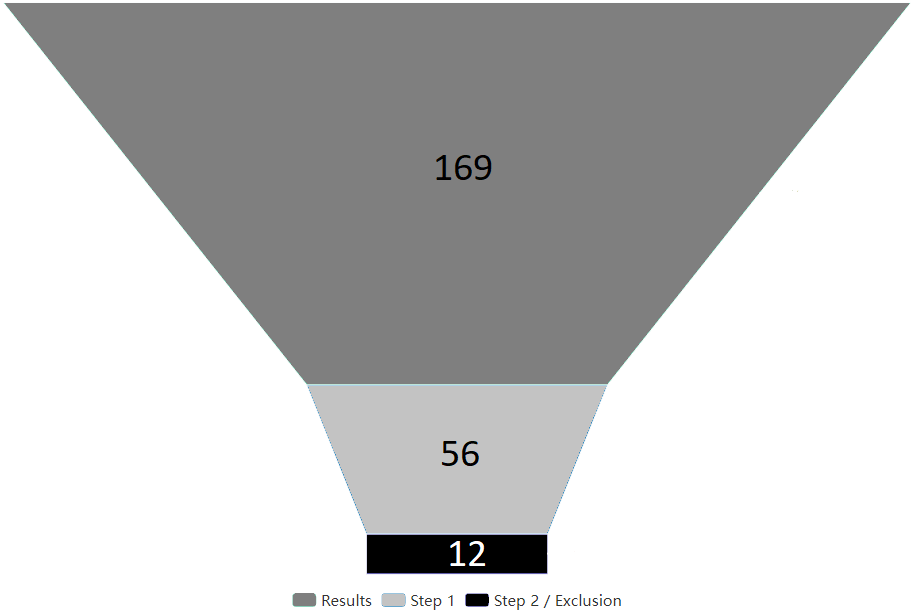
\includegraphics[width=12cm]{img/gl-results.png}
  \end{center}
  \fonte{Author.}
\end{figure}

\subsection{Data Extraction}\label{sec:gl-data-extraction}

In this section, it will be presented how the two data extractions from the found tools were performed, one for the feature matrix and another to retrieve more information on the most important features in common between the tools.

\subsubsection{Feature Matrix}\label{sec:gl-feature-matrix}

After the research was carried out, in order to apply the quality criteria, it was necessary to create a matrix of functionalities among the filtered results. In this way, the authors were able to understand which features are present most frequently among the evaluated tools. A total of 37 features were found, some repeating themselves more than others. The matrix can be seen in \Cref{fig:gl-matrix}.

\begin{figure}[!htb]
  \caption{Feature Matrix}\label{fig:gl-matrix}
  \begin{center}
    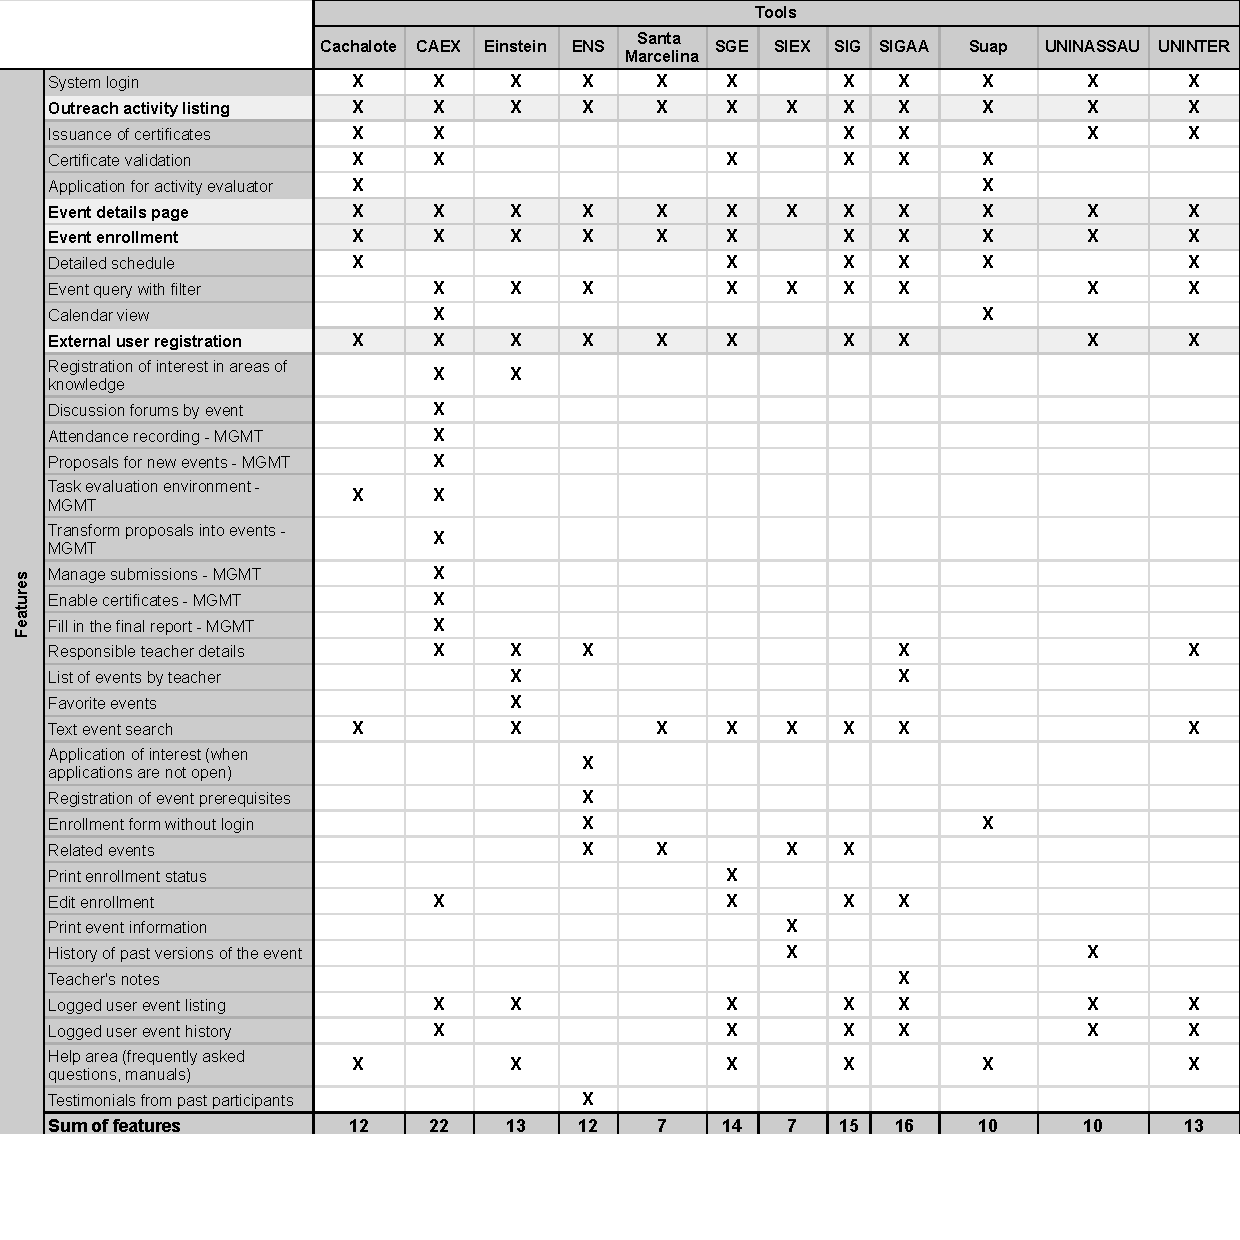
\includegraphics[width=16cm]{img/functionality-matrix.pdf}
  \end{center}
  \fonte{Author.}
\end{figure}

The most common features among all the evaluated tools and websites were highlighted in lighter grey, so that they could be used as criteria in the next phase of data extraction.

\subsubsection{More Information from Important Features}\label{sec:gl-data-extraction-2}

In the second data extraction, the objective was to identify which information was used in the
\begin{inparaenum}[(i)]
  \item Listing of outreach activities;
  \item Detailed page of an activity;
  \item Enrollment of a participant into an activity;
  \item Registration of users external to the institution.
\end{inparaenum}

Because each tool has its own attribute naming and its own format, it was difficult to standardize the analysis, so the original names were kept. Tools that did not have the selected features have been highlighted in grey instead of leaving the cells in blank, to avoid confusion. The extracted results are written in an informal way precisely because it was almost impossible to try to follow a pattern for all the tools. The extracted data can be seen in \Cref{fig:gl-additional-extraction}.

\begin{figure}[!htb]
  \caption{Additional Information Extraction}\label{fig:gl-additional-extraction}
  \begin{center}
    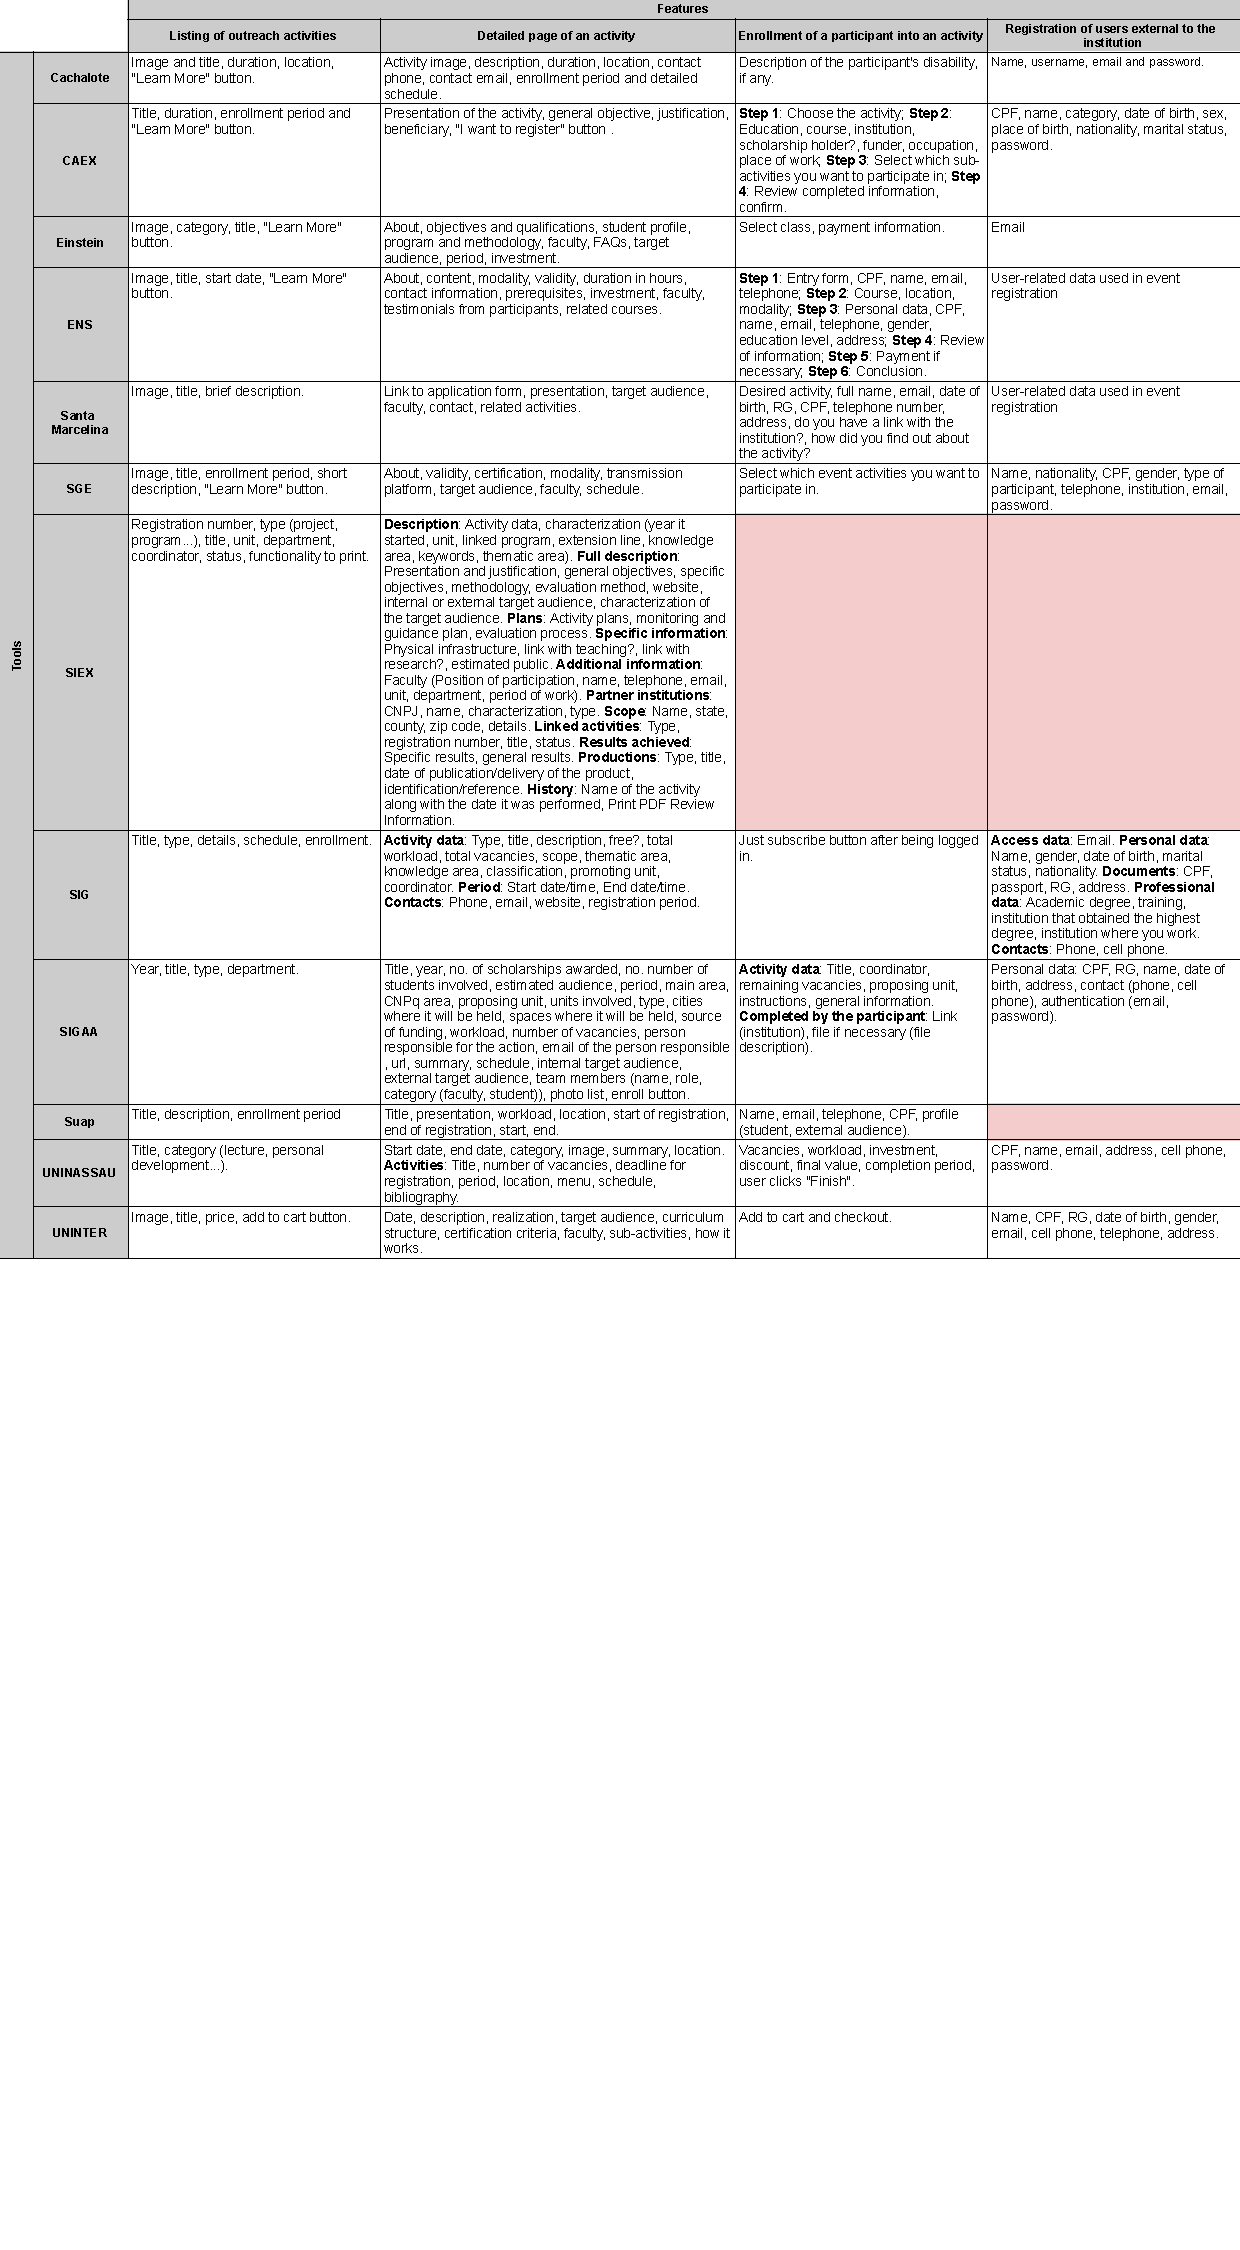
\includegraphics[width=16cm]{img/gl-data-extraction-2.pdf}
  \end{center}
  \fonte{Author.}
\end{figure}

\subsection{Tool Classification}\label{sec:gl-tool-classification}

Once all the data had been extracted and tabulated, it was possible to classify the tools using the previously defined quality criteria. 0 (zero) is the minimum and 5 (five) is the maximum score for a tool. The final results obtained are displayed in \Cref{tbl:gl-quality-criteria-results}.

\begin{table}
  \centering
  \caption{Quality Criteria Evaluation}
  \label{tbl:gl-quality-criteria-results}
  \arrayrulecolor{black}
  \scriptsize
  \begin{tabular}{c|p{2cm}|cc|cc|cc|cc|cc|c}
    \hhline{~~-----------}
    \multicolumn{2}{l}{\multirow{3}{*}{~ ~ ~ ~ ~ ~}}                                & \multicolumn{11}{c}{{\cellcolor[rgb]{0.753,0.753,0.753}}\textbf{Quality Criteria ~ ~ ~ ~ ~ ~ ~ ~}}                                                                                                                                                                                                                                                                                                                                                                                                                                                                                                                                                                                                                                                                                                                                                         \\
    \hhline{~~-----------}
    \multicolumn{2}{l}{}                                                            & \multicolumn{2}{c|}{{\cellcolor[rgb]{0.753,0.753,0.753}}\textbf{QC 1. ~}}                          & \multicolumn{2}{c|}{{\cellcolor[rgb]{0.753,0.753,0.753}}\textbf{QC 2. ~}} & \multicolumn{2}{c|}{{\cellcolor[rgb]{0.753,0.753,0.753}}\textbf{QC 3. ~}} & \multicolumn{2}{c|}{{\cellcolor[rgb]{0.753,0.753,0.753}}\textbf{QC 4. ~}} & \multicolumn{2}{c|}{{\cellcolor[rgb]{0.753,0.753,0.753}}\textbf{QC 5. }} & \multicolumn{1}{l}{{\cellcolor[rgb]{0.753,0.753,0.753}}}                                                                                                                                                                                                                                                                                                                                                                               \\
    \multicolumn{2}{l}{}                                                            & {\cellcolor[rgb]{0.753,0.753,0.753}}\textbf{Ans.}                                                  & {\cellcolor[rgb]{0.753,0.753,0.753}}\textbf{Score}                        & {\cellcolor[rgb]{0.753,0.753,0.753}}\textbf{Ans.}                         & {\cellcolor[rgb]{0.753,0.753,0.753}}\textbf{Score}                        & {\cellcolor[rgb]{0.753,0.753,0.753}}\textbf{Ans.}                        & {\cellcolor[rgb]{0.753,0.753,0.753}}\textbf{Score}       & {\cellcolor[rgb]{0.753,0.753,0.753}}\textbf{Ans.} & {\cellcolor[rgb]{0.753,0.753,0.753}}\textbf{Score} & {\cellcolor[rgb]{0.753,0.753,0.753}}\textbf{Ans.} & {\cellcolor[rgb]{0.753,0.753,0.753}}\textbf{Score} & \multicolumn{1}{l}{\multirow{-2}{*}{{\cellcolor[rgb]{0.753,0.753,0.753}}\begin{tabular}[c]{@{}l@{}}\textbf{Final}\\\textbf{Results }\end{tabular}}}       \\
    \hhline{>{\arrayrulecolor[rgb]{0.753,0.753,0.753}}-->{\arrayrulecolor{black}}-----------}
    \rowcolor[rgb]{0.898,0.898,0.898} {\cellcolor[rgb]{0.753,0.753,0.753}}          & {\cellcolor[rgb]{0.753,0.753,0.753}}\textbf{Cachalote}                                             & 9                                                                         & 0,0                                                                       & No                                                                        & 0,0                                                                      & 12                                                       & 0,5                                               & Partially                                          & 0,5                                               & 2021                                               & 0,5                                                                                                                                                 & 1,5 \\
    {\cellcolor[rgb]{0.753,0.753,0.753}}                                            & {\cellcolor[rgb]{0.753,0.753,0.753}}\textbf{CAEX}                                                  & 4                                                                         & 0,0                                                                       & 7                                                                         & 1,0                                                                      & 22                                                       & 1,0                                               & Yes                                                & 1,0                                               & 2022                                               & 1,0                                                                                                                                                 & 4,0 \\
    \rowcolor[rgb]{0.898,0.898,0.898} {\cellcolor[rgb]{0.753,0.753,0.753}}          & {\cellcolor[rgb]{0.753,0.753,0.753}}\textbf{Einstein}                                              & 12                                                                        & 0,5                                                                       & 1                                                                         & 0,5                                                                      & 13                                                       & 0,5                                               & Partially                                          & 0,5                                               & 2022                                               & 1,0                                                                                                                                                 & 3,0 \\
    {\cellcolor[rgb]{0.753,0.753,0.753}}                                            & {\cellcolor[rgb]{0.753,0.753,0.753}}\textbf{ENS}                                                   & 11                                                                        & 0,5                                                                       & 3                                                                         & 1,0                                                                      & 12                                                       & 0,5                                               & Partially                                          & 0,5                                               & 2022                                               & 1,0                                                                                                                                                 & 3,5 \\
    \rowcolor[rgb]{0.898,0.898,0.898} {\cellcolor[rgb]{0.753,0.753,0.753}}          & {\cellcolor[rgb]{0.753,0.753,0.753}}\textbf{Santa Marcelina}                                       & 6                                                                         & 0,0                                                                       & No                                                                        & 0,0                                                                      & 7                                                        & 0,0                                               & Partially                                          & 0,5                                               & 2022                                               & 1,0                                                                                                                                                 & 1,5 \\
    {\cellcolor[rgb]{0.753,0.753,0.753}}                                            & {\cellcolor[rgb]{0.753,0.753,0.753}}\textbf{SGE}                                                   & 8                                                                         & 0,0                                                                       & 1                                                                         & 0,5                                                                      & 14                                                       & 1,0                                               & Yes                                                & 1,0                                               & 2016                                               & 0,0                                                                                                                                                 & 2,5 \\
    \rowcolor[rgb]{0.898,0.898,0.898} {\cellcolor[rgb]{0.753,0.753,0.753}}          & {\cellcolor[rgb]{0.753,0.753,0.753}}\textbf{SIEX}                                                  & 53                                                                        & 1,0                                                                       & 1                                                                         & 0,5                                                                      & 7                                                        & 0,0                                               & Yes                                                & 1,0                                               & 2022                                               & 1,0                                                                                                                                                 & 3,5 \\
    {\cellcolor[rgb]{0.753,0.753,0.753}}                                            & {\cellcolor[rgb]{0.753,0.753,0.753}}\textbf{SIG}                                                   & 18                                                                        & 0,5                                                                       & No                                                                        & 0,0                                                                      & 15                                                       & 1,0                                               & Partially                                          & 0,5                                               & 2022                                               & 1,0                                                                                                                                                 & 3,0 \\
    \rowcolor[rgb]{0.898,0.898,0.898} {\cellcolor[rgb]{0.753,0.753,0.753}}          & {\cellcolor[rgb]{0.753,0.753,0.753}}\textbf{SIGAA}                                                 & 28                                                                        & 1,0                                                                       & 1                                                                         & 0,5                                                                      & 16                                                       & 1,0                                               & Yes                                                & 1,0                                               & 2022                                               & 1,0                                                                                                                                                 & 4,5 \\
    {\cellcolor[rgb]{0.753,0.753,0.753}}                                            & {\cellcolor[rgb]{0.753,0.753,0.753}}\textbf{Suap}                                                  & 8                                                                         & 0,0                                                                       & No                                                                        & 0,0                                                                      & 10                                                       & 0,5                                               & Yes                                                & 1,0                                               & 2022                                               & 1,0                                                                                                                                                 & 2,5 \\
    \rowcolor[rgb]{0.898,0.898,0.898} {\cellcolor[rgb]{0.753,0.753,0.753}}          & {\cellcolor[rgb]{0.753,0.753,0.753}}\textbf{UNINASSAU}                                             & 14                                                                        & 0,5                                                                       & No                                                                        & 0,0                                                                      & 10                                                       & 0,5                                               & Partially                                          & 0,5                                               & 2022                                               & 1,0                                                                                                                                                 & 2,5 \\
    \multirow{-12}{*}{{\cellcolor[rgb]{0.753,0.753,0.753}}\rotcell{\textbf{Tools}}} & {\cellcolor[rgb]{0.753,0.753,0.753}}\textbf{UNINTER}                                               & 9                                                                         & 0,0                                                                       & No                                                                        & 0,0                                                                      & 13                                                       & 0,5                                               & Partially                                          & 0,5                                               & 2022                                               & 1,0                                                                                                                                                 & 2,0 \\
    \toprule
  \end{tabular}

  \fonte{Author.}
\end{table}

With this classification, it is easy to see that the ``CAEX'' tool and ``\ac{SIGAA}'' achieved the highest grades, and this was really the expected result. First because ``\ac{SIGAA}'' is one of the most used academic management tools by institutions in the country and ``CAEX'' is the tool that presented the most unique features. Thus, being two tools with great potential and that contributed a lot in the acquisition of information to build the goal product.

\subsection{Answering the Research Questions}\label{sec:gl-answer-research-questions}

The \Cref{tab:research-questions} contains the research questions and was presented earlier in the study. However, each question is also described below, for the sake of convenience.

\begin{itemize}
  \item \textbf{RQ 1.} What tools currently exist that perform academic management?

        This is a question that in general also covers some tools that were removed in the application of inclusion and exclusion criteria. In this case 36 tools were found that supported academic management of some nature, but those that pass the criteria established, are listed in the tool matrix in \Cref{fig:gl-matrix}, totaling 12 tools.
  \item \textbf{RQ 1.1.} Which ones have related functionality or support outreach activities?

        As it was already shown in \Cref{fig:gl-matrix}, which describes the relations between tools and features, the following tools were discovered:
        \begin{inparaenum}[(1)]
          \item Cachalote;
          \item CAEX;
          \item Einstein;
          \item ENS;
          \item Santa Marcelina;
          \item SGE;
          \item SIEX;
          \item SIG;
          \item SIGAA;
          \item SUAP;
          \item UNINASSAU and
          \item UNINTER.
        \end{inparaenum}

  \item \textbf{RQ 1.2.} What are the features offered by these tools?

        All the features found were listed in the features matrix, present in \Cref{fig:gl-matrix}, with a total of 37 features.
  \item \textbf{RQ 1.3.} What are the most common features between this type of tool?

        The most common functionalities in this type of tool are:
        \begin{inparaenum}[(i)]
          \item A login system;
          \item Lististing of \aclp{OA};
          \item \ac{OA} details page;
          \item \ac{OA} enrollment and
          \item Registration of external users.
        \end{inparaenum}
        There is another feature that appears frequently but not as much as the others: the search for events by text, with 8 of the tools found implementing this functionality.
  \item \textbf{RQ 1.4.} What data do the tools use in relation to activities, participant registration and user registration?

        By analyzing the second data extraction presented in \Cref{sec:gl-data-extraction-2}, the most common fields for \acp{OA} are:
        \begin{inparaenum}[(a)]
          \item Title;
          \item Duration;
          \item Enrollment period;
          \item Contact information;
          \item Description;
          \item Target audience;
          \item Faculty and
          \item Schedule.
        \end{inparaenum}

        Regarding enrollment, the most common fields found are:
        \begin{inparaenum}[(a)]
          \item Participant's personal data;
          \item Institutional affiliation;
          \item Participant type and
          \item Information about the participant's disability, if any.
        \end{inparaenum}

        When it comes to user registration, basically personal data, authentication data and address are the most used by these tools, others also ask for information about the institution, type of participant and professional data.
\end{itemize}

\section{Validity}\label{sec:gl-validity}

During the stages of the systematic review mapping, some threats to validity were identified. Most of them the authors were able to minimize, but others remain unresolved. They are as follows:
\begin{itemize}
  \item During the research stage, the authors noticed that the search results varied minimally, between one or two different records when comparing the results they both obtained. It was an easy threat to mitigate, but it couldn't be completely ruled out. The strategy used was to log out of the account logged into the browser and perform the search in anonymous mode. This ended up reducing the number of divergences, but there were still cases of different results.
  \item Lack of validation of functionalities with the developers of the tools found. Unfortunately, the authors were unsuccessful in contacting any universities regarding the management solution being used.
  \item Related to conducting the research, in order to minimize the divergence of results, the authors tried to conduct the search in the shortest possible time, starting and completing it in just three days. If the delay was longer, there would be an increasing opportunity to bring threats to the study, as the search engine is considered a ``black box'', making it difficult to predict the exact results that will come with each search string.
\end{itemize}

\section{Considerations}\label{sec:gl-considerations}

Through this systematic review of the grey literature, it was possible to find tools similar to what the goal product of the whole study should be. Before conducting the review, there was no idea of the current state of the area and of which solutions are most widely used by Brazilian \ac{HEI}.

A lot of valuable information about tools being used today was collected. The scope of \aclp{OA} management and processes was now much clearer. This knowledge will make a difference when implementing the goal product, which aims to be an all around solution for \ac{OA} administration.

Also, all research questions that were previously defined in the review protocol could be answered.